\chapter{Implementation}

\section{Flow chart}

\begin{figure}[htb]
    \centering
    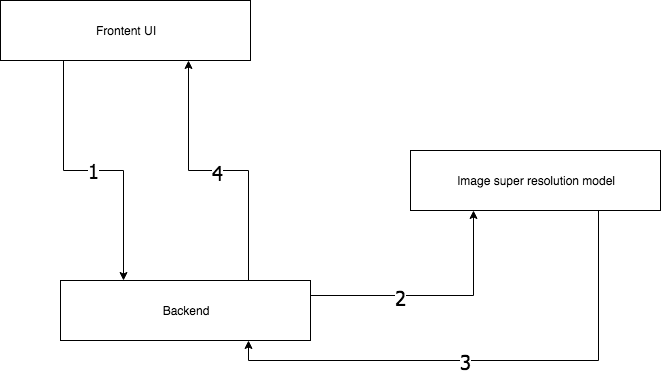
\includegraphics[width=\linewidth]{flow.png}
    \caption{Flow diagram}
    \label{fig:flow}
\end{figure}

\section {Overview of implementation}

The frontend is a React JavaScript app which provides a simple interface that allows user to upload any image in their computer or in their mobile device. The user uploaded image is then converted into a based64 encoded string and is passed on to the backend as a JSON through a POST request.

The backend is a Flask application that runs using Gunicorn. What we have in here is a simple web API that is expecting a POST request from the frontend with the content as the image that is to be converted and sent back. Flask provies us with a super simple and efficent API for creating web API's. Gunicorn lets up run Flask as a multithreaded web app handling all the multithreading heavylifing. When the backend recieves the image from the frontend as a API POST call from we convert that image from an bse64 encode string into a file.

This file is then fed into the Image super resolution model. The model is the core of the project and convets the image from a low resolution image into a high resolution image. This is done using a \textbf{Deep Denoiseing Super Resolution (DDSRCNN)} model. Once the model has done it's job of conveting the lower reolution image into a higher resolution image, it is sent back to the backend. The backend then encodes the new better image into a base64 encode string and sends it to the frontend.

The frontend service, once the result is received back from the bakend server will display that to the user and will have an option to download and store the image. The whole frontend is a completely static site which is hosted on a public static site hosting servie that is provide by surge.sh. The main advantage of hosting it on a public hosting service is that due to the availablility of CDN's (Content Delivery Network) arround the globe the page load speed will be very fast.

\section{Deep Denoiseing Super Resolution (DDSRCNN)}

The framework is fully convolutional (and deconvolutional. Deconvolution is essentially unsampling convolution). Rectification layers are added after each convolution and deconvolution. For low-level image restoration problems, we use neither pooling nor unpooling in the network as usually pooling discards useful image details that are essential for these tasks. It is worth mentioning that since the con- volutional and deconvolutional layers are symmetric, the network is essentially pixel-wise prediction, thus the size of input image can be arbitrary. The input and output of the network are images of the same size $w$ × $h$ × $c$, where $w$, $h$ and $c$ are width, height and number of channels.
Our main idea is that the convolutional layers act as a feature extractor, which preserve the primary components of objects in the image and meanwhile eliminating the corruptions. After forwarding through the convolutional layers, the corrupted input image is converted into a “clean” one. The subtle details of the image contents may be lost during this process. The deconvolutional layers are then combined to recover the details of image contents. The output of the deconvolutional layers is the recovered clean version of the input image. Moreover, we add skip connections from a convolutional layer to its corresponding mirrored deconvo- lutional layer. The passed convolutional feature maps are summed to the deconvolutional feature maps element-wise, and passed to the next layer after rectification. Deriving from the above architecture, we have used two networksvin our experiments, which are of 20 layers and 30 layers respectively, for image denoising, image super-resolution, JPEG deblocking and image inpainting.
\begin{figure}[htb]
    \centering
    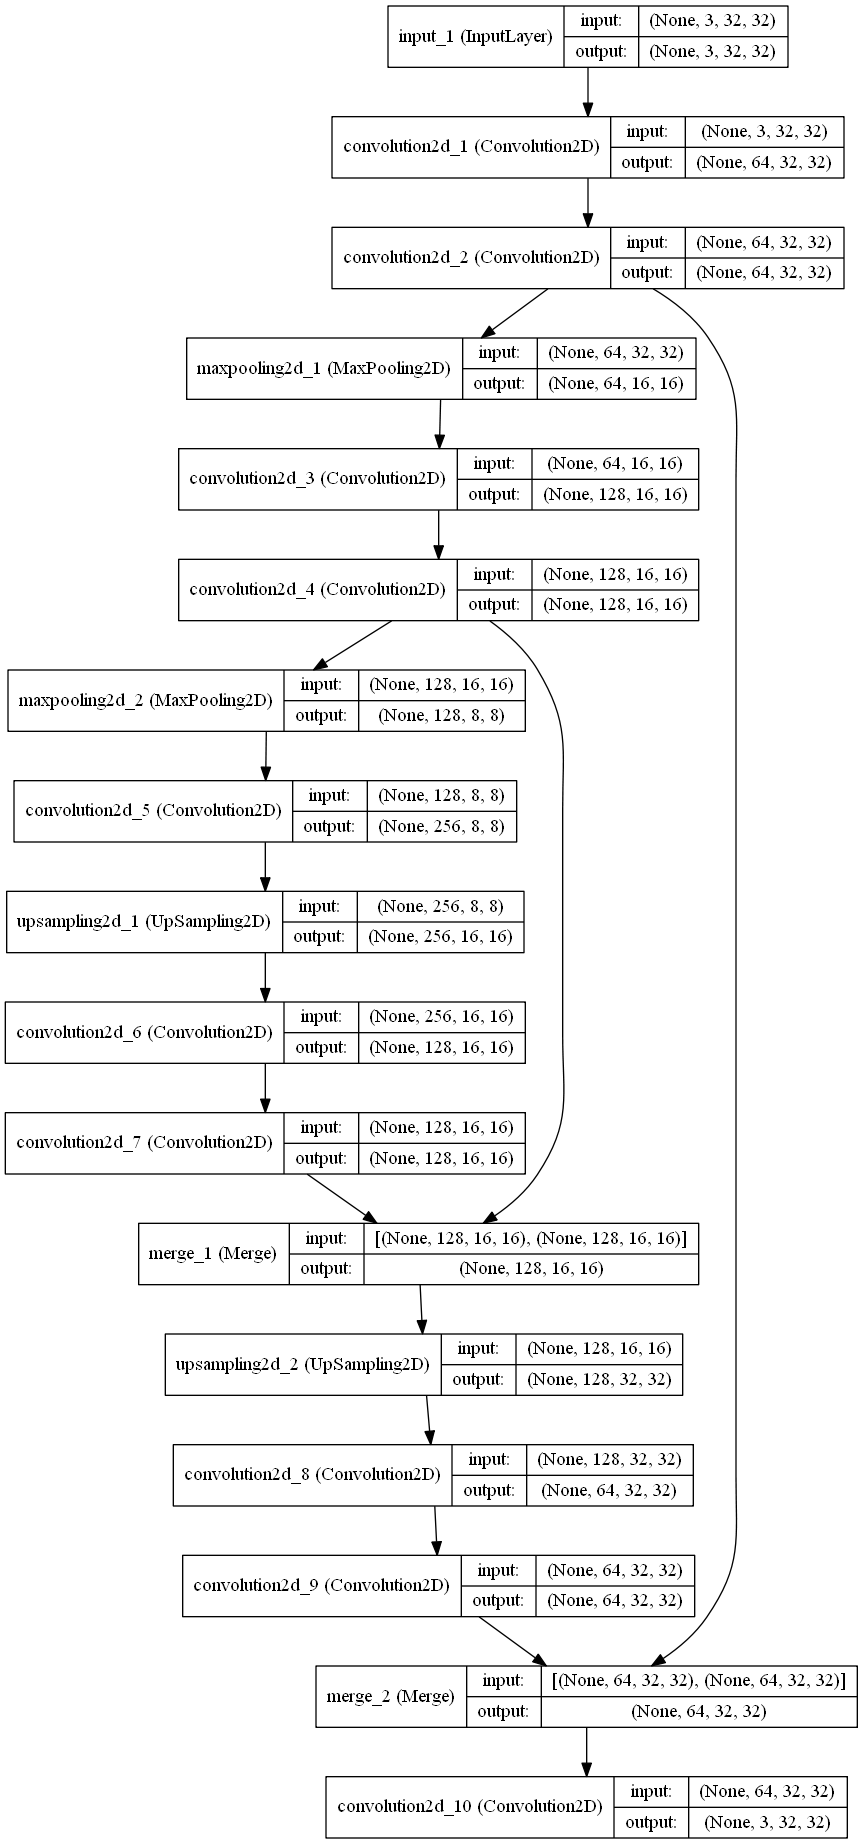
\includegraphics[width=\textwidth,height=15cm,keepaspectratio]{model.png}
    \caption{Deep Denoise model}
    \label{fig:modeldd}
\end{figure}
